\chapter{样板图样}\label{cha:xangmu1}
{\bfseries 知识目标}
\begin{itemize}
\item 了解国家制图标准和电气 AutoCAD 制图规范
\item 掌握平面图样的绘制步骤和方法
\item 掌握用 AutoCAD 绘制平面图样的基本步骤和方法
\item 掌握 AutoCAD 基本的绘图命令和编辑命令
\end{itemize}

{\bfseries 技能目标}
\begin{itemize}
\item 具备平面样抄绘能力
\item 具备使用AutoCAD绘制中等复杂程度的图样的能力
\item 具备阅读和分析平面图样的能力
\end{itemize}

{\bfseries 本章导引}

图\ref{fig:shangmu1}所示图纸即为图样,是根据投影法,并按照国家或国际标准的规定绘制的,用于工程施工或产品制造等用途的图。标准则是为了在一定范围内获得最佳秩序,而对活动或其结果规定共同的和重复使用的规则、导则或特性的文件。本章旨在通过讲解图\ref{fig:shangmu1}所示项目,使学生在完成项目的同时,了解和掌握国家制图标准中图幅、比例、线型、文字、标注等相关知识,以及通过AutoCAD进行图样绘制的步骤、方法、技巧和规范,并能运用所学的技巧和知识解决绘图过程中的实际问题,具备遵照国家制图标准和规范抄绘图样的能力。
\noindent
\begin{landscape}
\begin{figure}[htbp]
\centering
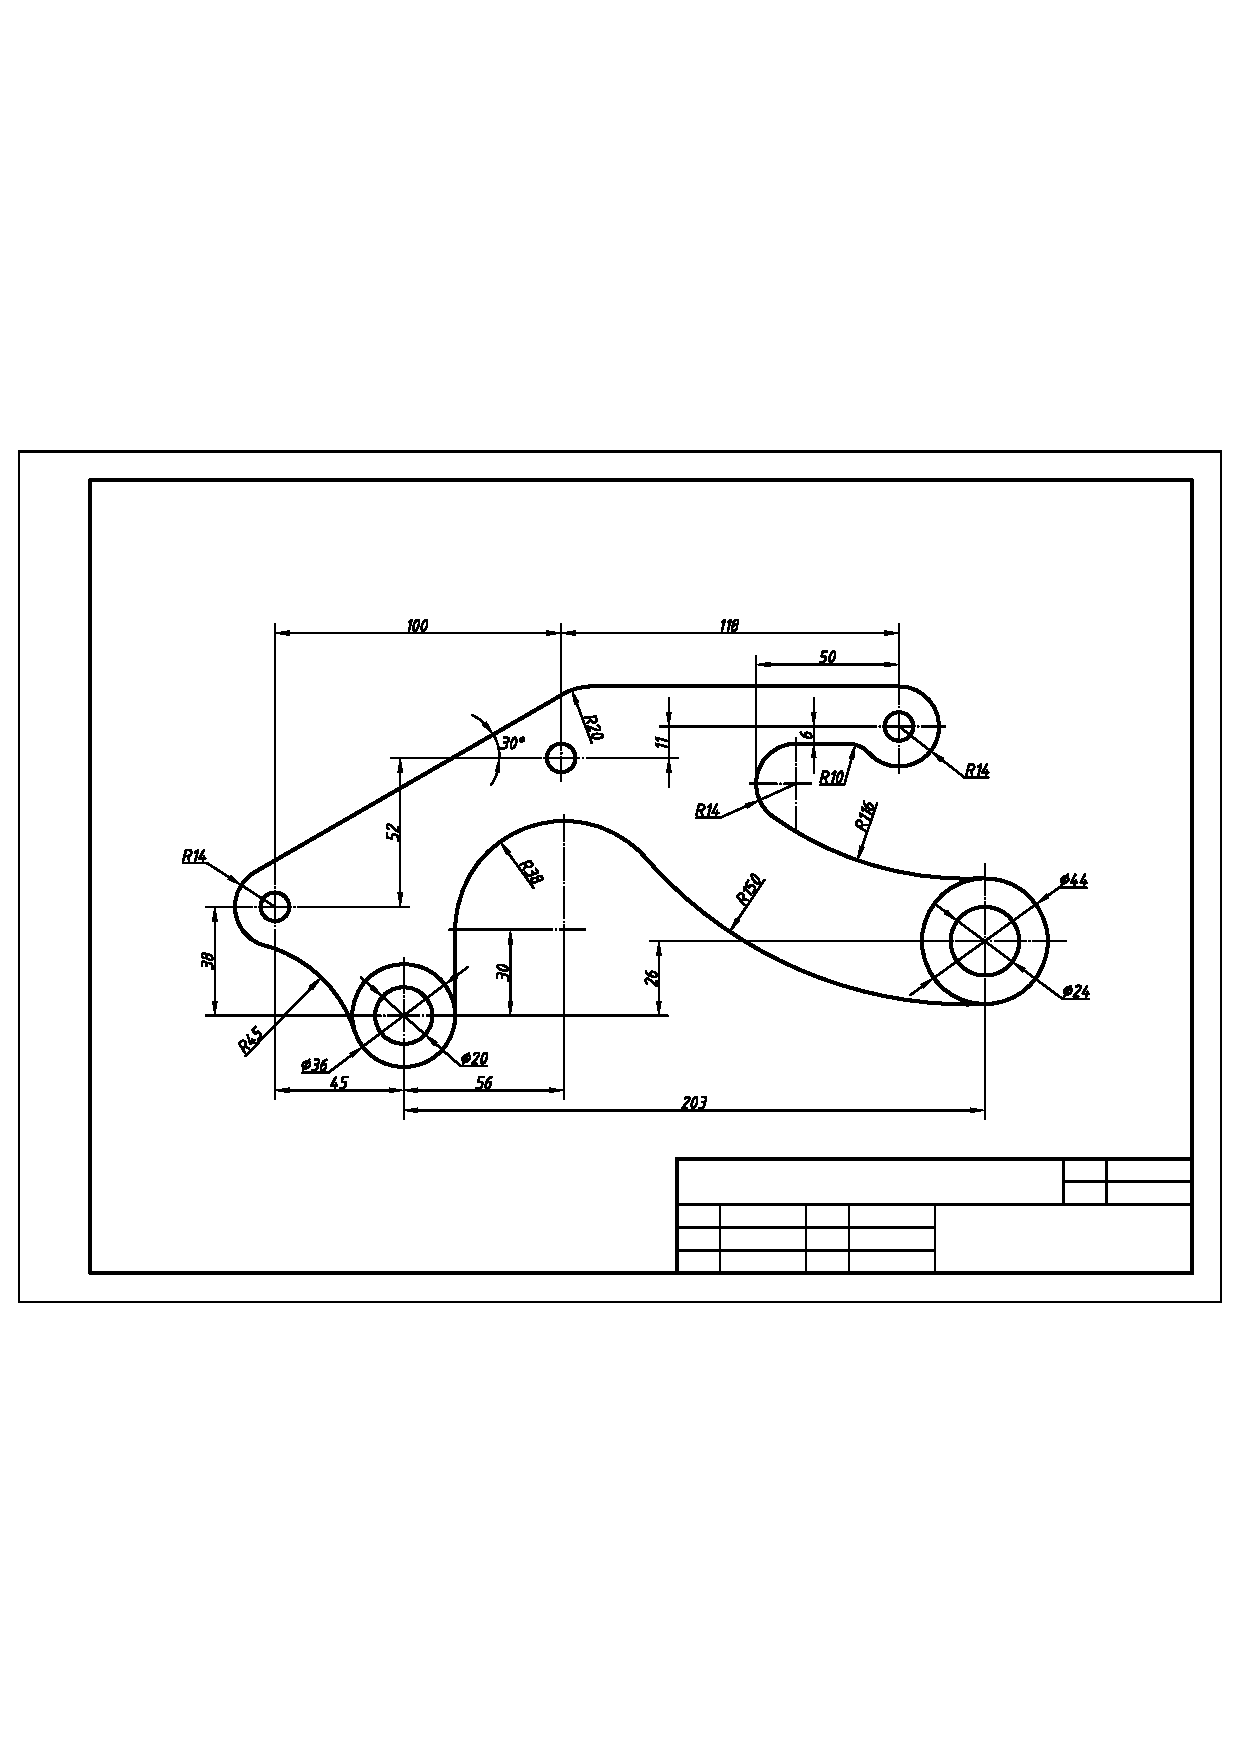
\includegraphics[scale=0.9]{fuzatuyang3.pdf}
\caption{项目一示例}\label{fig:shangmu1}
\end{figure}
\end{landscape}
\indent
%\newpage
\endinput





